\section{Einleitung}
In diesem Versuch werden mithilfe eines Germaniumdetektors die Spektren
unterschiedlicher radioaktiver Quellen untersucht. Anhand dieser Daten sollen unter Anderem
die Aktivität einer Quelle errechnet werden, oder die Isotope einer unbekannten Strahlequelle bestimmt
werden. Weiterhin soll die Vollenergienachweiswahrscheinlichkeit des Detektors bstimmt und die Merkmale eines Gammaspektrums untersucht werden.

\section{Theorie}


\subsection{Photonwechselwirkung in Materie}

Im Allgemeinen wird radioaktive Strahlung durch ihre Art der Entstehung und Reichweite unterschieden.
Dabei handelt es sich um $\alpha$-, $\beta$- und $\gamma$-Strahlung. In diesem Versuch wird $\gamma$-Strahlung
untersucht. Diese Art von ioniserender Strahlung wird von Atomkernen emittiert, die sich nach einem $\alpha$- oder
$\beta$-Zerfall in einem angeregten Zustand befinden. Beim Übergang von dem angeregten Zustand in den Grundzustand oder einen
weniger angeregten Zustand wird Energie in Form eines $\gamma$-Quants frei. Da es sich bei dem $\gamma$-Quant um ein
ungeladenes Teilchen handelt, wechselwirkt es deutlich weniger oft als beispielsweise die $\alpha$-Strahlung. Somit weist die
$\gamma$-Strahlung die höchste Eindringtiefe in Materie auf. \\
Je nach Energie wechselwirken die $\gamma$-Quanten dennoch mit der umliegenden Materie.
Die Abhängigkeit der Wechselwirkungsart von der Photonenernergie ist in Abbildung \ref{fig:WW}
dargestellt.
\begin{figure}[H]
    \centering
    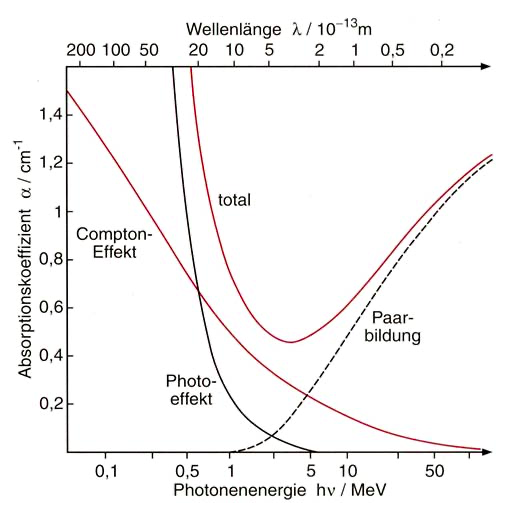
\includegraphics[width=0.8\textwidth]{WW.png}
    \caption{Energieabhängigkeit der Wechselwirkungsarten von Photonen mit Materie \cite{WW}.}
    \label{fig:WW}
\end{figure} \noindent
Wie in Abbildung \ref{fig:WW} zu erkennen ist, ist bei kleinen Energien der Photoeffekt der
dominate Wechselwirkungsprozess. Dabei sind eingestrahlte Photonen in der Lage, Elektronen aus
einem Metall zu lösen, wenn ihre Energie groß genug ist die materialspezifische Austrittsabeit
zu überwinden. Typische Austrittsarbeiten liegen im Bereich von einigen Elektronenvolt. So beträgt
die Austritssarbeit bei Caesium beispielsweise $\SI{1,94}{\electronvolt}$ und bei Germanium
ca. $\SI{5}{\electronvolt}$. Die Energie der Photonen, die über die Austrittsarbeit hinausgeht
führen die herausgelösten Elektronen in Form von kinetischer Energie
\begin{equation*}
    E_\text{kin} = E_\text{Photon} - W_\text{Austritt}
\end{equation*}
mit sich. Durch das Herauslösen des Elektrons bleibt ein Loch zurück, welches durch ein Elektron
aus einer höheren Schale gefüllt wird. Dabei wird Energie in Form von Röntgenstrahlung frei, die
jedoch im Material absorbiert wird. \\
In einem Energiebereich von ca.$\SI{100}{\kilo\electronvolt}$ bis $\SI{10}{\mega\electronvolt}$ dominiert
der Comptoneffekt. Beim Comptoneffekt wird das Photon an einem ruhenden Elektron gestreut.
Durch die Streuung kommt es zu einem Energieverlust und damit zu einer Vergrößerung der
Wellenlänge. Die Änderung der Wellenlänge ist dabei abhängig vom Streuwinkel zwischen Photon und
Elektron. Die Wahrscheinlichkeit für das Auftreten der Compton-Streuung wird durch den
Klein-Nishina-Wirkungsquerschnitt angegeben. Dieser gibt dabei die Winkelverteilung der gestreuten
Photonen an.
Der differentielle Wirkungsquerschnitt in Abhängigkeit der Energie und dem Streuwinkel $\phi$ ist durch
\begin{equation*}
    \frac{d\sigma}{d\Omega} = \frac{1}{2} \frac{\alpha^2}{m^2} \left(\frac{E'}{E}\right)^2 \left[\frac{E'}{E}+\frac{E}{E'}-\sin(\phi)^2\right]
\end{equation*} \noindent
gegeben. Wobei $E'$ der Energie des gestreuten und E der Energie des eingestrahlten Photons entspricht.

Die Energie des gestreuten Photons lässt sich mit
\begin{equation}
  E' = \frac{E}{1+\frac{E}{m_\text{e}c^2}(1-\cos(\phi))}
  \label{eqn:Compton}
\end{equation}
berechnen.
Die Energie des Elektrons beträgt also $E_\text{e} = E-E'\,$.
Die Comptonkante beschreibt die maximale Energie, die ein gestreutes Photon an das Elektron abgeben kann.
Dies geschieht bei einem Streuwinkel von $\phi = \SI{180}{\degree}$.
Die Lage der Comptonkante liegt somit bei
\begin{equation}
  E_\text{Kante} = \frac{E \cdot \frac{2E}{m_\text{e}c^2}}{1+\frac{2E}{m_\text{e}c^2}} \, .
  \label{eqn:Comptonkante}
\end{equation}

Die Lage des Rückstreupeaks ist durch die Energie
\begin{equation}
  E_\text{Rück.} = E - E_\text{Kante}
  \label{eqn:Compton_Rückstreupeak}
\end{equation}
beschrieben, die ein mit $\SI{180}{\degree}$ gestreutes Photon in dem Detektor abgeben kann.

Die Intensiät von Photonen in Abhängigkeit der Energie $E$ und der Eindringtiefe $x$ in das Material, kann durch das Lambert-Beer’sche Gesetz

\begin{equation}
  I(E,x) = I_0 \cdot e^{-\mu(E) x}
  \label{eqn:Lambert}
\end{equation}

bestimmt werden. Dabei beschreibt $\mu(E)$ den linearen Abschwächungskoeffizienten des Materials. Dieser setzt sich  aus den Abschwächungskoeffizienten für Photoeffekt, Comptoneffekt und Paarbildung zusammen.

\subsection{Detektor}

Der Germaniumdetektor ist ein Halbleiterdetektor. Er besteht aus einer p- und einer n-dotierten Schicht, die aneinandergrenzen.
Die freien Löcher und Elektronen in der p- und n-Schicht rekombinieren in der Grenzschicht und es entsteht eine ladungsträgerarme Zone (Verarmungszone oder Sperrschicht).

Dringt ein Gammaquant in die Sperrschicht ein, wechselwirkt es mit den dort befindlichen Elektronen.
So können durch ein Gammaquant mehrere Elektronen ins Leitungsband gehoben werden und dort selbst, durch Stöße, weitere Elektronen ins Leitungsband heben. Im Valenzband bleiben damit Löcher zurück.
So entstehen Elektronen-Loch-Paare, die sich bei Anlegen einer Spannung getrennt an den Elektroden ansammeln und einen Ladungsimpuls erzeugen.
Dieser ist proportional zur Anzahl der erzeugten Elektron-Loch-Paare und somit proportional zur deponierten Energie des Gammaquant.

Die Dicke der Sperrschicht muss möglichst groß gewählt werden, um die Anzahl der Wechselwirkungen zu erhöhen.
Durch eine höhere Spannung und eine unsymmetrische Dotierung steigt die Dicke der Sperrschicht.
Eine hohe Spannung beschleunigt allerdings Elektronen, welche durch hohe thermische
Energien in das Leitungsband gehoben wurden.
Dadurch steigt die Untergrundrate des Detektors.
Um den Einfluss der thermischen Effekte gering zu halten, wird der Detektor mit flüssigem Stickstoff gekühlt.

Ein typisches Spektrum eines monoenergetischen Strahlers ist in Abbildung \ref{fig:Theorie-Spektrum} zu sehen.
Es lässt sich in die folgenden Merkmale unterteilen:
\begin{description}
  \item[Photopeak] Wird die gesamte Energie des Gammaquant über den Photoeffekt absorbiert, entsteht ein Peak bei der Energie des Gammaquant, da alle, über den Photoeffekt wechselwirkenden Photonen, die selbe Energie deponieren. \\
  \item[Compton-Kontinuum] Das Compton-Kontinuum erstreckt sich über den gesamten Energiebereich, der durch die Compton-Streuung im Detektormaterial deponiert werden kann. \\
  \item[Comptonkante] Maximale Energieabgabe des Gammaquant durch eine Streuung von $\SI{180}{\degree}$ im Detektormaterial.\\
  \item[Rückstreupeak] Wird das Gammaquant im Detektormantel um $\SI{180}{\degree}$ gestreut, ist die Energie des Rückstreupeaks die maximale Energie, die das Gammaquant danach im Detektor deponieren kann.
  \item[$\symbf{E >} \text{Comptonkante}$] Bei schnell aufeinander folgende Streuungen des Gammaquant kann der Detektor diese nicht auseinander halten. Somit kommt es zu Messwerten bei Energien, die größer sind als die der Comptonkante.
\end{description}

\begin{figure}[H]
  \centering
  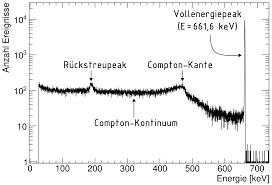
\includegraphics[width = .7\textwidth]{Theorie-spektrum.png}
  \caption{Typisches Spektrum einer monoenergetischen Quelle \cite{Theorie-Spektrum}.}
  \label{fig:Theorie-Spektrum}
\end{figure}

\subsection{Vollenergienachweiswahrscheinlichkeit}
Die Vollenergienachweiswahrscheinlichkeit gibt die Wahrscheinlichkeit an, mit der ein Photon seine gesamte Energie in dem Detektor deponiert.
Sie ist somit der Quotient aus den Photonen, die in dem Detektor ihre gesamte Energie im Photopeak deponieren, und denen, die in den Detektor gelangen.
\begin{equation*}
  Q(E) = \frac{N_\text{det.}}{N_\text{ein}}
\end{equation*}

Die Photonenanzahl $N_\text{ein}$ lässt sich aus der Aktivität $A$ der Quelle, der Emissionswahrscheinlichkeit $W$ der Photonenernergie, der Messzeit $T_\text{M}$ und dem, durch den Detektor abgedeckten, Raumwinkel $\Theta$ mit
\begin{equation*}
  N_\text{ein} = A \frac{\Theta}{4 \pi} T_\text{M} W
\end{equation*}
berechnen.
Die Anzahl $N_\text{det.}$ wird aus dem Peakinhalt zur zugehörigen Emissionsenergie bestimmt.
Für die Vollenergienachweiswahrscheinlichkeit folgt somit
\begin{equation}
  Q(E) = \frac{N_\text{det.}(E)}{A \frac{\Theta}{4 \pi} T_\text{M} W(E)}
  \label{eqn:Vollenergienachweiswahrscheinlichkeit}
\end{equation}

\section{Aufbau}
Der Germaniumdetektor ist zylinderförmig und hat eine, durch Eindiffusion von Lithium, n-dotierte Oberfläche.
Im Innern befindet sich eine mit Gold bedampfte koaxiale Bohrung, sodass dort eine starke p-Dotierung vorliegt.
An die Innen- und Außenseite des Detektors wird eine Hochspannung angelegt.
Um den Detektor herum befindet sich eine Aluminumhülle zum Schutz.
Die Kühlung des Detektors wird durch einen großen Stickstofftank gewährleistet, dieser ist über einen Temperaturfühler mit dem Detektor verbunden.
Der Temperaturfühler greift in die Elektronik ein und verhindert ein Einschalten der Hochspannung bei zu hohen Temperaturen, da dann der Detektor zerstört werden würde.
Die gemessenen Signale werden, linear zu der gemessenen Spannung, von einem Vielkanalanalysator den Kanälen zugeordnet.

In Abbildung \ref{fig:Aufbau} ist eine schematische Skizze des Detektors abgebildet.
Der eigentliche Detektor hat einen Durchmesser von $d = \SI{45}{\milli\meter}$ und eine Länge von $l=\SI{39}{\milli\meter}$.
Für viele Rechnungen ist der, vom Detektor abgedeckte, Raumwinkel $\Theta$ wichtig.
Dieser lässt sich aus dem Abstand zwischen Detektoroberfläche und Quelle, sowie dem Durchmesser des Detektors berechnen.
Zuerst kann der volle Öffnungswinkel $\varphi$ des gerade Kegels, der als Grundfläche die Obefläche des Detektors und als Spitze die Quellposition hat, mit

\begin{equation*}
  \varphi = 2\arctan\left(\frac{\sfrac{d}{2}}{l}\right)
\end{equation*}

berechnet werden \cite{wiki:Kegelwinkel}.
Aus diesem folgt mit
\begin{equation}
  \Theta = 2 \pi (1-\cos(\varphi))
  \label{eqn:Raumwinkel}
\end{equation}
der Raumwinkel $\Theta$ \cite{wiki:Theta}. Der Raumwinkel der gesamten Raumes beträgt $4\pi$.

\begin{figure}[H]
  \centering
  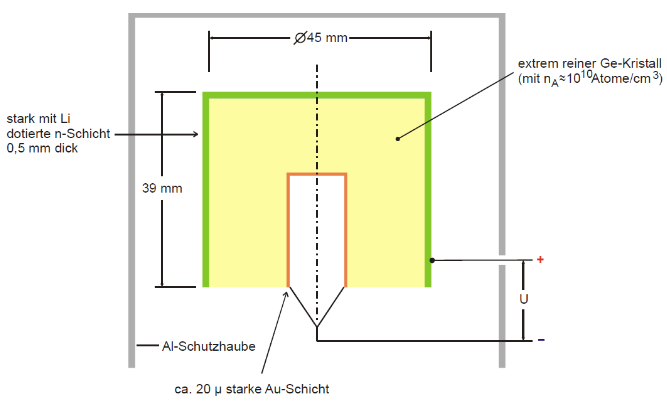
\includegraphics[width = .7\textwidth]{Aufbau.png}
  \caption{Aufbau des Germaniumdetektors \cite{Aufbau}.}
  \label{fig:Aufbau}
\end{figure}

\section{Durchführung}
An dem gekühlten Detektor werden \SI{5}{\kilo\volt} angelegt.
Die Probe wird über dem Detektor eingespannt und die Messung über einen Computer, welcher mit einem Vielkanalanalysator verbunden ist, gestartet.
Es wird eine \ce{^152Eu}, eine \ce{^137Cs} und eine \ce{^133Ba} bei einer Messzeit von einer halben Stunde vermessen.
Danach wird eine unbekannte Quelle in Form eines Steins für zwei Stunden vermessen. Auf eine Untergrundmessung wird verzichtet, da das Untergrundsignal für höhere Energien schnell abnimmt und größtenteils nur Photopeaks analysiert werden, deren Höhe weit oberhalb des Untergrundsignals liegt. 
